\documentclass{article}
\usepackage[utf8]{inputenc}
\usepackage{geometry}
\usepackage{graphicx}
\usepackage{amsmath}
\usepackage{amsfonts}
\usepackage{amsthm}
\usepackage{amssymb}
\usepackage[most]{tcolorbox}
\usepackage{array}
\usepackage{latexsym}
\usepackage{alltt}
\usepackage{hyperref}
\usepackage{color}
\usepackage{float}
\usepackage{pdfpages}
\usepackage{algpseudocode}
\usepackage{multicol}
\usepackage{multirow}
\usepackage{caption}
\usepackage{xparse}
\usepackage{setspace}
\usepackage{enumitem}
\usepackage{pdflscape}


\geometry
{
  a4paper,
  left=15mm,
  right=15mm,
  top=15mm,
  bottom=15mm,
}

% mybox
\newtcolorbox{mybox}[3][]
{
  colframe = #2!25,
  colback  = #2!10,
  coltitle = #2!20!black,  
  title    = {#3},
  #1,
}

% New environments that use mybox

\newcounter{example}
\newenvironment{example}[1]{\begin{mybox}[breakable]{green}{\refstepcounter{example}\textbf{Example~\theexample #1}}}{\end{mybox}}

\newenvironment{examplebreak}[1]{\begin{mybox}[breakable]{green}{\refstepcounter{example}\textbf{Example~\theexample #1}}}{\end{mybox}}

\newcounter{definition}[section]
\newenvironment{definition}[1]{\refstepcounter{definition}\begin{mybox}[breakable]{blue}{\textbf{Definition \thesection.\thedefinition #1}}}{\end{mybox}}

\newcounter{theorem}[section]
\newenvironment{theorem}[1]{\begin{mybox}{red}{\refstepcounter{theorem}\textbf{Theorem \thesection.\thetheorem #1}}}{\end{mybox}}

\newenvironment{formula}[1]{\begin{mybox}{cyan}{\textbf{#1}}}{\end{mybox}}

% Changing maketitle
\makeatletter         
\renewcommand\maketitle{
{\raggedright % Note the extra {
\begin{center}
{\Large \bfseries \@title}\\[2ex] 
{\large \@author \ - \@date}\\[2ex]
\end{center}}} % Note the extra }
\makeatother

% \onehalfspacing % adjust spacing
\setlength{\parskip}{0.5\baselineskip}

% macros
\newcommand{\prob}[1]{\textbf{\textit{P}}\{#1\}}
\NewDocumentCommand{\dsum}{%
    e{^_}
}{%
  {% 
    \displaystyle\sum
    \IfValueT{#1}{^{#1}}
    \IfValueT{#2}{_{#2}}
  }
}%

% maketitle variables
\title{CENG 280 - Review}
\author{Burak Metehan Tunçel}
\date{April 2022}

\begin{document}

\maketitle

\section{Chapter 1}

\begin{multicols}{2}
\setlength{\columnsep}{1.5cm}
\setlength{\columnseprule}{0.2pt}

\subsection{Alphabets and Languages}

\textbf{Alphabet:} A finite set of symbols, e.g., $\{a, b, \ldots, z\}$, $\{0, 1\}$.

\textbf{String:} A string over an alphabet is a finite sequence of symbols from the alphabet, e.g., ``$0011$'', ``$a$'', ``$e$'' (empty string). The set of all strings (including the empty string) over $\Sigma$ is denoted by $\Sigma^*$. The length of a string is the length of the sequence, e.g. $|abc| = 3$.

\textbf{Language:} Any subset $L$ of $\Sigma^*$ for an alphabet $\Sigma$ is called a language over $\Sigma$.

\subsubsection{String Operations}

\textbf{Concatenation:} Two strings $x$, $y$ over the same alphabet, e.g. $x, y \in \Sigma^*$, can be combined. $w = x \circ y$, or simply $w = xy$.

\textbf{Substring:} A string $v$ is a substring of $w$ if $w$ can be written as $w = xvy$. If $w = vx$ then $v$ is a \textit{prefix} of $w$, and if $w = xv$, then $v$ is a \textit{suffix} of $w$.

\textbf{Reversal:} The reverse of a string $w$, denoted by $w^R$, is the string spelled backwards. For example, $w = abc \Rightarrow w^R = cba$.

\begin{theorem}{}
  For any two strings $x, w$, $(wx)^R = x^Rw^R$.
\end{theorem}

\subsubsection{Languages}

Given an alphabet $\Sigma$, any subset of $\Sigma^*$ is called a language.
\begin{equation*}
  L = \left\{ w \in \Sigma^*\ |\ w \textnormal{ has the property } P \right\}
\end{equation*}

\paragraph{Language Operations}

Languages are sets, so set operations (union, intersection, difference) can be used on languages.
\begin{itemize}
  \item \textbf{Complement:} $\overline{L} = \Sigma^* \setminus L$
  \item \textbf{Concatenation:} $L_1, L_2$ are languages over $\Sigma$. $L = L_1 \circ L_2$ (or simply $L = L_1L_2$) is defined as
    \begin{equation*}
      L = \left\{ w_1w_2\ |\ w_1 \in L_1 \textnormal{ and } w_2 \in L_2 \right\}
    \end{equation*}
  \item \textbf{Kleene star:} The Kleene star of a language $L$, denoted by $L^*$, is the set of strings obtained by concatenating $0$ or more strings from $L$.
  \item $L^+ = LL^*$  
\end{itemize}

\vfill\null
\columnbreak

\subsection{Finite Representations of Languages}

\begin{definition}{: Regular Expression}
  The regular expressions over an alphabet $\Sigma$ are all strings over the alphabet $\Sigma \cup \{( , ), \emptyset, \cup, *\}$ that can be obtained as follows:
  \begin{enumerate}
    \item $\emptyset$ and each member of $\Sigma$ is a regular expression.
    \item If $\alpha$ and $\beta$ are regular expressions than so is $(\alpha\beta)$.
    \item If $\alpha$ and $\beta$ are regular expressions than so is $(\alpha \cup \beta)$.
    \item If $\alpha$ is a regular expression than so is $\alpha^*$.
    \item Nothing is a regular expression unless it follows from 1-4.
  \end{enumerate}
\end{definition}

\textit{\textbf{Every regular expression defines a language.}}

\begin{definition}{: Languages defined by regular expressions}
  For a regular expression $\alpha$, $L(\alpha)$ is the language represented by $\alpha$ and it is defined as
  \begin{enumerate}
    \item $L(\emptyset) = \emptyset$ and $L(a) = \left\{ a \right\}$ for each $a \in \Sigma$.
    \item If $\alpha$ and $\beta$ are regular expressions than $L(\alpha\beta) = L(\alpha)L(\beta)$.
    \item If $\alpha$ and $\beta$ are regular expressions than $L(\alpha \cup \beta) = L(\alpha) \cup L(\beta)$.
    \item If $\alpha$ is a regular expression than so is $L(\alpha^*) = L(\alpha)^*$
  \end{enumerate}
\end{definition}

The class of \textbf{regular languages} consists of all languages $L$ such that $L = L(\alpha)$ for some regular expression $\alpha$.

\noindent \textbf{Language recognition device:} For some language $L$, an algorithm that answers the question is $w \in L$

\noindent \textbf{Language generators:} Descriptions of how a string from a language can be produced.

\end{multicols}


\newpage
\section{Chapter 2}

\begin{multicols}{2}
\setlength{\columnsep}{1.5cm}
\setlength{\columnseprule}{0.2pt}

\subsection{DFA: Deterministic Finite Automata}

\begin{definition}{}
  A \textbf{deterministic finite automaton} is a quintuple $M = (K, \Sigma, \delta, s, F)$ where
  \begin{itemize}
    \item $K$ is a finite set of \textbf{states}
    \item $\Sigma$ is an alphabet,
    \item $s \in K$ is the \textbf{initial state}
    \item $F \subseteq K$ is the set of \textbf{final states}
    \item $\delta$, the \textbf{transition function}, is a function from $K \times \Sigma$ to $K$. 
  \end{itemize}
\end{definition}

The \textbf{configuration} of the machine is the \textit{current state and the unread part of the input string}, i.e., a configuration is an element of $K \times \Sigma^*$.

Let $(q, w)$ and $(q',w')$ be two configurations of $M$. Then $(q, w) \vdash_M (q', w')$ if and only if $w = aw'$ for some $a \in \Sigma$ and $q' = \delta(q, a)$. For example, $(q, aabb) \vdash_M (q', abb)$ where $q' = \delta(q, a)$.

$(q, w) \vdash_M (q', w')$ reads $(q, w)$ \textbf{yields} $(q', w')$ in \textbf{one step}. $\vdash^*_M$ is the \textbf{reflexive transitive closure} of $\vdash_M$ (It can be though like the multiple steps). A string $w \in \Sigma^*$ is \textbf{accepted} by $M$ if and only if $(s, w) \vdash^*_M (f, e)$ for some $f \in F$. The \textbf{language} of $M$, $L(M)$, is the set of strings \textit{accepted} by $M$.

\vfill\null
\columnbreak


\subsection{NFA: Nondeterministic Finite Automata}

\begin{definition}{}
  A \textbf{nondeterministic finite automaton} is a quintuple $M = (K, \Sigma, \Delta, s, F)$, where
  \begin{itemize}
    \item $K$ is a finite set of \textbf{states}
    \item $\Sigma$ is an alphabet
    \item $s \in K$ is the \textbf{initial state}
    \item $F \subseteq K$ is the set of \textbf{final states}, and
    \item $\Delta$, the \textbf{transition relation}, is a subset of $K \times (\Sigma \cup \{e\}) \times K$ 
\end{itemize}
\end{definition}

$(q, a, p) \in \Delta$ is called a \textbf{transition} of $M$. $(q, e, p)$ indicates that the machine can pass to state $p$ from state $q$ without reading an input symbol.

The \textbf{configuration} of the machine is the current state and the unread part of the input string, i.e., a configuration is an element of $K \times \Sigma^*$.

Let $(q, w)$ and $(q', w')$ be two configurations of $M$. Then $(q, w) \vdash_M (q', w')$ if and only if $w = aw'$ for some $a \in \Sigma \cup \{e\}$ and $(q, a, q') \in \Delta$.

$(q, w) \vdash_M (q', w')$ reads $(q, w)$ \textbf{yields} $(q', w')$ \textbf{in one step}. $\vdash^*_M$ is the \textbf{reflexive transitive closure} of $\vdash_M$. $(q, w) \vdash^*_M (q', w')$ reads $(q, w)$ yields $(q', w')$. A string $w \in \Sigma^*$ is \textbf{accepted} by $M$ if and only if there is a state $f \in F$ such that $(s, w) \vdash^*_M (f, e)$. The \textbf{language} of $M$, $L(M)$, is the set of strings accepted by $M$.

\textit{A deterministic finite state automaton is just a special type of nondeterministic finite state automaton}. We obtain a DFA when $\Delta$ defines a function from $K \times \Sigma$ to $K$. In other words, an NFA $M = (K, \Sigma, \Delta, s, F)$ is deterministic if there are no transitions of the form $(q, e, p)$ and for each $q \in K$ and $a \in \Sigma$, there exists \textit{exactly one} $p \in K$ such that $(q, a, p) \in \Delta$.

A nondeterministic finite automaton can always be converted to an \textit{equivalent} deterministic finite state automaton.

\begin{theorem}{}
  For each nondeterministic finite automaton, there exists an equivalent deterministic finite automaton.
\end{theorem}

Proof of the theorem is constructive. In proof, one can use subset construction algorithm to construct a DFA from anNFA and then show they are equivalent.

Two automaton (DFA or NFA, one can be DFA and the other can be NFA) $M_1$ and $M_2$ are said to be \textbf{equivalent} when $L(M_1) = L(M_2)$.

\end{multicols}

\newpage
\subsubsection{Subset Construction}

In here, the following is main and formal definition.

\begin{formula}{}
Given an NFA $M = (K, \Sigma, \Delta, s, F)$, the algorithm constructs an equivalent DFA $M' = (K', \Sigma, \delta, s', F')$ as follows. For each state $q \in K$, the set of states that can be reached without reading an input symbol is defined as
  \begin{align*}
    E(q) = \left\{ p \in K\ |\ (q, e) \vdash^*_M (p, e) \right\}
  \end{align*}
  Essentially, $E(q)$ is the reflexive transitive closure of the set $\left\{ q \right\}$ under the relation $\left\{(p, r)\ |\ (p, e, r) \in \Delta \right\}$. The DFA is defined as:
  \begin{align*}
    K' &= 2^K\\
    s' &= E(s)\\
    F' &= \left\{ Q \subseteq K\ |\ Q \cap F \neq \emptyset \right\}\\
    \delta'(Q, a) &= \left\{ E(p) : p \in K, (q, a, p) \in \Delta \textnormal{ for some } q \in Q \right\} \textnormal{ for each $Q \in K'$ and $a \in \Sigma$}\\
    &= \bigcup \left\{ E(p) : p \in K, (q, a, p) \in \Delta \textnormal{ for some } q \in Q \right\}
  \end{align*}
\end{formula}

\begin{multicols}{2}
\setlength{\columnsep}{1.5cm}
\setlength{\columnseprule}{0.2pt}

\begin{equation*}
  E(q) = \left\{ q \right\} \cup \left\{ p \in K\ |\ (q, e) \vdash^*_M (p, e) \right\}
\end{equation*}

If there is question about transforming an NFA to a DFA, the following steps can be used in question solving:
\begin{formula}{}
  \begin{enumerate}
    \item The NFA $M = (K, \Sigma, \Delta, s, F)$ is given and we want to construct DFA. In other words we want to acquire:
    \begin{equation*}
        M' = (K', \Sigma, \delta', s', F')
    \end{equation*}
    
    \item Start from the initial state of NFA, $s' = E(s)$. For each $q_j \in E(s)$ find the transition for each $k \in \Sigma$ ($q_j, k, q_l$).

    For example, if $E(s) = \{ q_{0}, q_{1} \}$. Look the transition from $q_0$ and $q_1$. If $\Sigma = \{ a, b \}$, then look for $a$ and $b$.
    
    
    \item Then calculate the union of $E(q_i)$ of the reachable states from the state we consider.
    
    For example, if transitions for $a$ are $(q_{0}, a, q_{1}), (q_{1}, a, q_{2})$, then write 
    \begin{quote}
      $(q_{0}, a, q_{1}), (q_{1}, a, q_{2})$ are all the transitions $(q, a, p)$ for some $q \in E(s)$
    \end{quote}
    and calculate the $\delta'(s', a) = E(q_{1}) \cup E(q_{2})$. If it is new state, write this new state on DFA, if not connect it the old one.
    
    \item Follow this steps for each $k \in \Sigma$ and newly introduced steps.
  \end{enumerate}
\end{formula}

\vfill\null
\columnbreak

Look at the example below, it is taken from 2.2.4 in the textbook.

\begin{example}{: NFA to DFA}
  For this example:
  \begin{itemize}
    \item $E(q_0) = \left\{ q_0, q_1, q_2, q_3  \right\}$
    \item $E(q_1) = \left\{ {q_1, q_2, q_3} \right\}$
    \item $E(q_2) = \left\{ q_2 \right\}$
    \item $E(q_3) = \left\{ q_3 \right\}$
    \item $E(q_4) = \left\{ q_3, q_4 \right\}$
  \end{itemize}
  
  \hfill\break

  $s' = E(q_0) = \left\{ q_0, q_1, q_2, q_3  \right\}$,
  \begin{equation*}
    (q_1, a, q_0),\ (q_1, a, q_4), \textnormal{ and } (q_3, a, q_4)
  \end{equation*}
  are all the transitions $(q, a, p)$ for some $q \in s'$. It follows that (Instead of $s'$ any state symbol can be used such as $q_{100}$)
  \begin{equation*}
    \delta'(s', a) = E(q_0) \cup E(q_4) = \left\{ q_0, q_1, q_2, q_3, q_4 \right\}
  \end{equation*}
  Similarly,
  \begin{equation*}
    (q_0, b, q_2) \textnormal{ and } (q_2, b, q_4)
  \end{equation*}
  are all the transitions of the form $(q, b, p)$ for some $q \in E(q_0)$, so
  \begin{equation*}
    \delta'(s', b) = E(q_2) \cup E(q_4) = \left\{ q_2, q_3, q_4 \right\}
  \end{equation*}
  
  In here $\left\{ q_0, q_1, q_2, q_3, q_4 \right\}$ and $\left\{ q_2, q_3, q_4 \right\}$ are new states.
  
  Repeat this calculation for the newly introduced states. In the end, there will be no new states or you will be in wrong way.
\end{example}


\subsection{Finite Automata and Regular Expressions}

\begin{theorem}{}
  The class of languages accepted by finite automata is closed under
  \begin{enumerate}[label=\alph*)]
    \item union
    \item concatenation
    \item Kleene star
    \item complementation
    \item intersection
  \end{enumerate}
\end{theorem}

Let $M_1 = (K_1, \Sigma, \Delta_1, s_1, F_1)$ and $M_2 = (K_2, \Sigma, \Delta_2, s_2, F_2)$ be nondeterministic finite automata.

\begin{enumerate}[label=(\alph*)]
  % (a) Union
  \item \textit{Union.}
  $L(M) = L(M_1) \cup L(M_2)$.
  
  $M = (K, \Sigma, \Delta, s, F)$, where $s$ is a new state not in $K_1$ or $K_2$,
  \begin{itemize}
    \item $K = K_1 \cup K_2 \cup \left\{ s \right\}$
    \item $F = F_1 \cup F_2$
    \item $\Delta = \Delta_1 \cup \Delta_2 \cup \left\{ (s,e,s_1),(s,e,s_2) \right\}$
  \end{itemize}

  % (b) Concatenation
  \item \textit{Concatenation.}
  $L(M) = L(M_1) L(M_2)$.

  Then the finite automaton $M$ that accepts $L(M_1) L(M_2)$ is defined as follows (\textit{May include mistakes}). $M = (K, \Sigma, \Delta, s, F)$
  \begin{itemize}
    \item $s = s_1$
    \item $K = K_1 \cup K_2$
    \item $F = F_2$
    \item $\Delta = \Delta_1 \cup \Delta_2 \cup \left\{ (f,e,s_2)\ |\ f \in F_1 \right\}$
  \end{itemize}

  % (c) Kleenestar
  \item \textit{Kleene star.}
  $L(M) = L(M_1)^*$. 

  Then the finite automaton $M$ that accepts $L(M_1)^*$ is defined as follows (\textit{May include mistakes}). $M = (K, \Sigma, \Delta, s, F)$, where $s$ is not in $M_1$
  \begin{itemize}
    \item $K = K_1 \cup \left\{ s \right\}$
    \item $F = F_1 \cup \left\{ s \right\}$
    \item $\Delta = \Delta_1 \cup \left\{ (s,e,s_1) \right\}$
  \end{itemize}

  % (d) Complementation
  \item \textit{Complementation.}
  $\overline{L} = \Sigma^* - L(M)$. $\overline{M}$ is identical to $M$ except that final and non final states are interchanged.

  $M = (K, \Sigma, \Delta, s, F)$.
  \begin{itemize}
    \item $s = s_1$
    \item $K = K_1$
    \item $F = K \setminus F_1$
    \item $\Delta = \Delta_1$
  \end{itemize}

  % (e) Intersection
  \item \textit{Intersection.}
  \begin{equation*}
    L(M) = L(M_1) \cap L(M_2) = \overline{\overline{L(M_1)} \cup \overline{L(M_2)}}
  \end{equation*}
\end{enumerate}

% \vfill\null
% \columnbreak

\begin{theorem}{}
  \textit{A language is regular if and only if it is accepted by a finite automaton.}
\end{theorem}

\subsubsection{Converting FA to RE}

There are two popular methods for converting a DFA to its regular expression:
\begin{itemize}
  \item Arden's Method
  \item State elimination method
\end{itemize}
Arden's Method is a little more complicated. Consider the state elimination method to convert FA to RE.

\paragraph{Rules}

The rules for state elimination method are as follows
\begin{enumerate}
  \item \textit{The initial state of FA must not have any incoming edge.}

    If there is any incoming edge to the initial edge, then create a new initial state having no incoming edge to it.
  
  \item \textit{There must exist only one final state in FA.}
  
    If there exist multiple final states, then convert all the final states into non-final states and create a new single final state.
  
  \item \textit{The final state of DFA must not have any outgoing edge.}
  
    If this exists, then create a new final state having no outgoing edge from it.
  
  \item \textit{Eliminate all intermediate states one by one.}
\end{enumerate}

% \vfill\null
% \columnbreak

\begin{examplebreak}{}
  Get the regular expression from the following FA:
  \begin{center}
    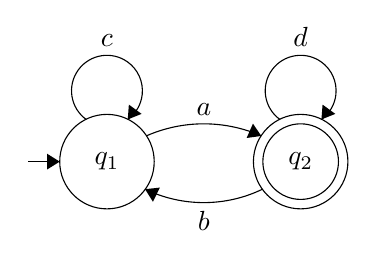
\begin{tikzpicture}[scale=0.2]
    \tikzstyle{every node}+=[inner sep=0pt]
    \draw [black] (5.2,-9.1) circle (3);
    \draw (5.2,-9.1) node {$q_1$};
    \draw [black] (17.5,-9.1) circle (3);
    \draw (17.5,-9.1) node {$q_2$};
    \draw [black] (17.5,-9.1) circle (2.4);
    \draw [black] (0.2,-9.1) -- (2.2,-9.1);
    \fill [black] (2.2,-9.1) -- (1.4,-8.6) -- (1.4,-9.6);
    \draw [black] (7.7,-7.466) arc (113.70628:66.29372:9.079);
    \fill [black] (15,-7.47) -- (14.47,-6.69) -- (14.07,-7.6);
    \draw (11.35,-6.2) node [above] {$a$};
    \draw [black] (15.081,-10.848) arc (-64.17666:-115.82334:8.565);
    \fill [black] (7.62,-10.85) -- (8.12,-11.65) -- (8.56,-10.75);
    \draw (11.35,-12.2) node [below] {$b$};
    \draw [black] (3.877,-6.42) arc (234:-54:2.25);
    \draw (5.2,-1.85) node [above] {$c$};
    \fill [black] (6.52,-6.42) -- (7.4,-6.07) -- (6.59,-5.48);
    \draw [black] (16.177,-6.42) arc (234:-54:2.25);
    \draw (17.5,-1.85) node [above] {$d$};
    \fill [black] (18.82,-6.42) -- (19.7,-6.07) -- (18.89,-5.48);
    \end{tikzpicture}
  \end{center}
  
  \textbf{Step 1:}
    
  Initial state $q_1$ has an incoming edge so create a new initial state $q_i$.
  \begin{center}
    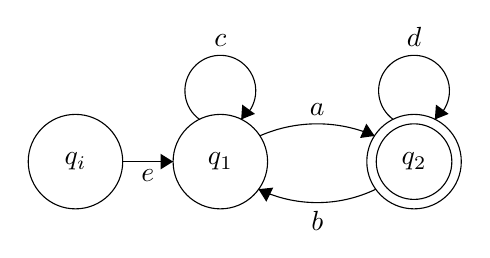
\begin{tikzpicture}[scale=0.2]
    \tikzstyle{every node}+=[inner sep=0pt]
    \draw [black] (12.4,-9.1) circle (3);
    \draw (12.4,-9.1) node {$q_1$};
    \draw [black] (24.7,-9.1) circle (3);
    \draw (24.7,-9.1) node {$q_2$};
    \draw [black] (24.7,-9.1) circle (2.4);
    \draw [black] (3.2,-9.1) circle (3);
    \draw (3.2,-9.1) node {$q_i$};
    \draw [black] (14.9,-7.466) arc (113.70628:66.29372:9.079);
    \fill [black] (22.2,-7.47) -- (21.67,-6.69) -- (21.27,-7.6);
    \draw (18.55,-6.2) node [above] {$a$};
    \draw [black] (22.281,-10.848) arc (-64.17666:-115.82334:8.565);
    \fill [black] (14.82,-10.85) -- (15.32,-11.65) -- (15.76,-10.75);
    \draw (18.55,-12.2) node [below] {$b$};
    \draw [black] (11.077,-6.42) arc (234:-54:2.25);
    \draw (12.4,-1.85) node [above] {$c$};
    \fill [black] (13.72,-6.42) -- (14.6,-6.07) -- (13.79,-5.48);
    \draw [black] (23.377,-6.42) arc (234:-54:2.25);
    \draw (24.7,-1.85) node [above] {$d$};
    \fill [black] (26.02,-6.42) -- (26.9,-6.07) -- (26.09,-5.48);
    \draw [black] (6.2,-9.1) -- (9.4,-9.1);
    \fill [black] (9.4,-9.1) -- (8.6,-8.6) -- (8.6,-9.6);
    \draw (7.8,-9.6) node [below] {$e$};
    \end{tikzpicture}
  \end{center}
  
  \textbf{Step 2:}
  
  Final state $q_2$ has an outgoing edge. So, create a new final state $q_f$.

  \begin{center}
    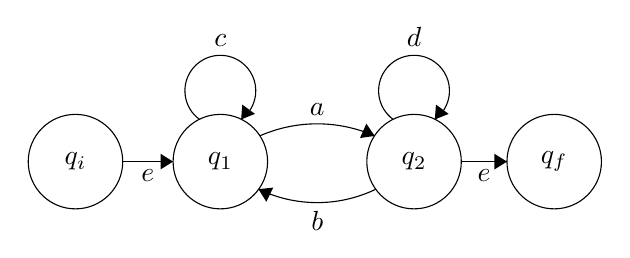
\begin{tikzpicture}[scale=0.2]
    \tikzstyle{every node}+=[inner sep=0pt]
    \draw [black] (12.4,-9.1) circle (3);
    \draw (12.4,-9.1) node {$q_1$};
    \draw [black] (24.7,-9.1) circle (3);
    \draw (24.7,-9.1) node {$q_2$};
    \draw [black] (3.2,-9.1) circle (3);
    \draw (3.2,-9.1) node {$q_i$};
    \draw [black] (33.6,-9.1) circle (3);
    \draw (33.6,-9.1) node {$q_f$};
    \draw [black] (14.9,-7.466) arc (113.70628:66.29372:9.079);
    \fill [black] (22.2,-7.47) -- (21.67,-6.69) -- (21.27,-7.6);
    \draw (18.55,-6.2) node [above] {$a$};
    \draw [black] (22.281,-10.848) arc (-64.17666:-115.82334:8.565);
    \fill [black] (14.82,-10.85) -- (15.32,-11.65) -- (15.76,-10.75);
    \draw (18.55,-12.2) node [below] {$b$};
    \draw [black] (11.077,-6.42) arc (234:-54:2.25);
    \draw (12.4,-1.85) node [above] {$c$};
    \fill [black] (13.72,-6.42) -- (14.6,-6.07) -- (13.79,-5.48);
    \draw [black] (23.377,-6.42) arc (234:-54:2.25);
    \draw (24.7,-1.85) node [above] {$d$};
    \fill [black] (26.02,-6.42) -- (26.9,-6.07) -- (26.09,-5.48);
    \draw [black] (6.2,-9.1) -- (9.4,-9.1);
    \fill [black] (9.4,-9.1) -- (8.6,-8.6) -- (8.6,-9.6);
    \draw (7.8,-9.6) node [below] {$e$};
    \draw [black] (27.7,-9.1) -- (30.6,-9.1);
    \fill [black] (30.6,-9.1) -- (29.8,-8.6) -- (29.8,-9.6);
    \draw (29.15,-9.6) node [below] {$e$};
    \end{tikzpicture}
  \end{center}

  \textbf{Step 3:}

  Start eliminating intermediate states

  \textbf{First eliminate $q_1$:}

  \quad There is a path going from $q_i$ to $q_2$ via $q_1$. So, after eliminating $q_1$ we can connect a direct path from $q_i$ to $q_2$ having cost: $e c^* a = c^* a$.

  \quad There is a loop on $q_2$ using state $q_i$. So, after eliminating $q_1$ we put a direct loop to $q_2$ having cost: $b c^* a$.

  After eliminating $q_1$, the FA looks like following
  \begin{center}
    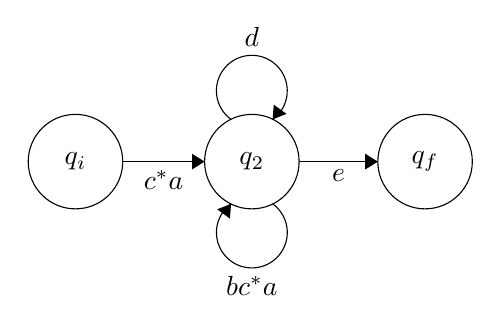
\begin{tikzpicture}[scale=0.2]
    \tikzstyle{every node}+=[inner sep=0pt]
    \draw [black] (14.4,-9.1) circle (3);
    \draw (14.4,-9.1) node {$q_2$};
    \draw [black] (3.2,-9.1) circle (3);
    \draw (3.2,-9.1) node {$q_i$};
    \draw [black] (25.4,-9.1) circle (3);
    \draw (25.4,-9.1) node {$q_f$};
    \draw [black] (13.077,-6.42) arc (234:-54:2.25);
    \draw (14.4,-1.85) node [above] {$d$};
    \fill [black] (15.72,-6.42) -- (16.6,-6.07) -- (15.79,-5.48);
    \draw [black] (17.4,-9.1) -- (22.4,-9.1);
    \fill [black] (22.4,-9.1) -- (21.6,-8.6) -- (21.6,-9.6);
    \draw (19.9,-9.6) node [below] {$e$};
    \draw [black] (6.2,-9.1) -- (11.4,-9.1);
    \fill [black] (11.4,-9.1) -- (10.6,-8.6) -- (10.6,-9.6);
    \draw (8.8,-9.6) node [below] {$c^*a$};
    \draw [black] (15.723,-11.78) arc (54:-234:2.25);
    \draw (14.4,-16.35) node [below] {$bc^*a$};
    \fill [black] (13.08,-11.78) -- (12.2,-12.13) -- (13.01,-12.72);
    \end{tikzpicture}
  \end{center}

  \textbf{Second eliminate $q_2$:}
  There is a direct path from $q_i$ to $q_f$ so, we can directly eliminate $q_2$ having cost.
  \begin{equation*}
    c^*a (d + bc^*a)^* e = c^*a (d + bc^*a)^*
  \end{equation*}
  which is our final regular expression for given finite automata.

\end{examplebreak}

\vfill\null
\columnbreak


\subsection{Languages that are and are not Regular}

To show that a language $L$ is regular, one of the following methods can be used:
\begin{itemize}
  \item write a regular expression $\alpha$ such that $L = L(\alpha)$
  \item construct an NFA $M$ such that $L = L(M)$
  \item use closure properties, e.g., for regular languages $L_1$ and $L_2$, show $L = L_1 \cap L_2$, $L = L_1 \cup L_2$, $L = L_1 L_2$,
  or $L = \Sigma^* \setminus L_1$ (more examples can be added)
\end{itemize}

There are two properties shared by all regular languages, but not by certain nonregular languages, may be phrased intuitively as follows: 
\begin{enumerate}
  \item As a string is scanned left to right, the amount of memory that is required in order to determine at the end whether or not the \textit{string is in the language must be bounded}, fixed in advance and dependent on the language, not the particular input string. For example, we would expect that $\{a^n b^n\ |\ n \geq 0\}$ is not regular, since it is difficult to imagine how a finite-state device could be constructed that would correctly remember, upon reaching the border between the $a$'s and the $b$'s, how many $a$'s it had seen, so that the number could be compared against the number of $b$'s.
  \item Regular languages with an infinite number of strings are represented by automata with cycles and regular expressions involving the Kleene star. Such languages must have infinite subsets with a certain simple repetitive structure that arises from the Kleene star in a corresponding regular expression or a cycle in the state diagram of a finite automaton. This would lead us to expect, for example, that $\{a^n\ |\ n \geq 1 \textnormal{ is a prime}\}$ is not regular, since there is no simple periodicity in the set of prime numbers.
\end{enumerate}

\noindent In brief,
\begin{formula}{}
  To show that a language $L$ is not regular, we use the following property of regular languages: 
  \begin{itemize}
    \item as a string is scanned from left to right, the amount of memory required to determine if $w \in L$ or $w \notin L$ must be bounded.
    \item In RL, infinite languages can be represented with Kleene star (cycle in automata), which induce a periodicity/pattern.
  \end{itemize}
\end{formula}

\end{multicols}

\newpage

\subsubsection{Pumping Lemma}

These intuitive ideas are formalized in the following theorem known as \textit{Pumping Lemma}.

\begin{theorem}{: Pumping Lemma}
  Let $L$ be a regular language. There is an integer $n \geq 1$ such that any string $w \in L$ with $|w| \geq n$ can be rewritten as $w = xyz$ such that $y \neq e$, $|xy| \leq n$ and $xy^iz \in L$ for each $i \geq 0$. 
\end{theorem}

\begin{formula}{}
  \quad Assume $L$ is a regular language and there is a string $w \in L$. Now, imagine, not find or determine, that there is a integer $n$ that is $n \geq 1$, $n > 0$. Also, this integer is smaller than the length of the string $w$, $n \leq |w|$. So,
\begin{align*}
  |w| \geq n \geq 1 && \textnormal{or} && |w| \geq n > 0
\end{align*}
Also, notice that the string can be written as three parts: $w = xyz$.

If the followings are satisfied, it shows that $w \in L$ and $L$ is regular:
\begin{itemize}
  \item $|y| > 0$: $y$ is not empty string
  \item $|xy| \leq n$: the length of the part of the string $xy$ is less than $n$
  \item $xy^iz \in L,\textnormal{ for each } i \geq 0$: When part $y$ is repeated, or pumped, as many times we want, the expression is still in language
\end{itemize}
In here, $x$ or $z$ can be empty string, $e$, but $y$ cannot be the empty string, $e$. Notice that the chosen part of string that will be compared with $n$ should be located in first $n$.
\end{formula}

Pumping lemma is also used to show that a language is not regular: start applying the pumping lemma, then find a contradiction.
\begin{formula}{}
\noindent For each regular language $L$,

\quad there exists $n \geq 1$ such that (this is a general term do not pick a number!!!)

\quad \quad for each $w \in L$ with $|w| \geq n$ (write/pick a string with respect to $n$, that can be used to reach a contradiction)

\quad \quad \quad there exists $x, y, z$ with $w = xyz$, $y \neq e$, $|xy| \leq n$ (consider each possible split satisfying these constraints)

\quad \quad \quad \quad for each $i \geq 0$, $xy^iz \in L$ (show that there exists an $i$ such that $xy^iz \neq L$, contradiction)
\end{formula}


\subsection{State Minimization}

The process of reducing a given DFA to its minimal form is called as minimization of DFA.
\begin{itemize}
  \item It contains the minimum number of states.
  \item The DFA in its minimal form is called as a Minimal DFA.
\end{itemize}

\noindent The two popular methods for minimizing a DFA are
\begin{itemize}
  \item Equivalence Theorem
  \item Myhill Nerode Theorem
\end{itemize}

\noindent Since Myhill Nerode Theorem is a little bit cumbersome and prone to error compared to Equivalence Theorem, it is better to focus on the Equivalence Theorem.

\newpage
\subsubsection{Equivalence Theorem}

\begin{multicols}{2}
\setlength{\columnsep}{1.5cm}
\setlength{\columnseprule}{0.2pt}

The steps as follows:
\begin{enumerate}
  % Step 1
  \item Eliminate all the dead states and inaccessible states from the given DFA (if any).
    \begin{itemize}
      \item \textbf{Dead State:} All those non-final states which transit to itself for all input symbols in $\Sigma$ are called as dead states.
      \item \textbf{Inaccessible State:} All those states which can never be reached from the initial state are called as inaccessible states.
    \end{itemize}
  
  % Step 2
  \item Draw a state transition table for the given DFA. Transition table shows the transition of all states on all input symbols in $\Sigma$.
  
  % Step 3
  \item Now, start applying equivalence theorem.
    \begin{itemize}
      \item Take a counter variable $k$ and initialize it with value 0.
      \item Divide $Q$ (\textit{set of states}) into two sets such that one set contains all the non-final states and other set contains all the final states.
      \item This partition is called $P_0$.
    \end{itemize}
  
  % Step 4
  \item 
    \begin{itemize}
      \item Increment $k$ by $1$.
      \item Find $P_k$ by partitioning the different sets of $P_{k - 1}$.
      \item In each set of $P_{k - 1}$, consider all the possible pair of states within each set and if the two states are distinguishable, partition the set into different sets in $P_k$.
    \end{itemize}
  
    Two states $q_1$ and $q_2$ are distinguishable in partition $P_k$ for any input symbol `$a$', if $\delta(q_1, a)$ and $\delta(q_2, a)$ are in different sets in partition $P_{k-1}$.
  
  % Step 5
  \item Repeat \textit{step-4} until no change in partition occurs. In other words, when you find $P_k = P_{k - 1}$, stop.
  
  % Step 6
  \item All those states which belong to the same set are equivalent. The equivalent states are merged to form a single state in the minimal DFA.
    \begin{center}
      \textit{\# of states in Minimal DFA = \# of sets in $P_k$  }
    \end{center}
\end{enumerate}

\end{multicols}


\section{Chapter 3: Discrete Random Variables and Their Distributions}

\begin{multicols}{2}
\setlength{\columnsep}{1.5cm}
\setlength{\columnseprule}{0.2pt}

\subsection{Distribution of Random Variable}

\subsubsection{Main Concepts}

\begin{itemize}
  \item A \textbf{random variable} is a function of an outcome,
    \begin{equation*}
        X = f(\omega)
    \end{equation*}
    In other words, it is a quantity that depends on chance.
  
  \item Collection of all the probabilities related to $X$ is the \textbf{distribution} of $X$. 
  
  \item \textbf{Probability Mass Function}, or \textbf{PMF}:
    \begin{equation*}
      P(x) = \prob{X = x}
    \end{equation*}
  
  \item \textbf{Cumulative Distribution Function}, or \textbf{CDF}:
    \begin{equation*}
        F(x) = \prob{X \leq x} = \sum_{y \leq x} P(y)
    \end{equation*}
  
  \item The set of possible values of $X$ is called the \textbf{support} of the distribution $F$.
  
  \item For every outcome $\omega$, the variable $X$ takes one and only one value $x$. This makes events $\{X = x\}$ disjoint and exhaustive, and therefore,
  \begin{equation*}
      \sum_x P(x) = \sum_x \prob{X = x} = 1
  \end{equation*}
\end{itemize}

\subsubsection{Types of Random Variables}

\begin{itemize}
  \item \textit{Discrete random variables}:
    
    These are variables whose range is \textit{finite or countable}. In particular, it means that their values can be listed, or arranged in a sequence. Examples include the number of jobs submitted to a printer, the number of errors, the number of error-free modules, the number of failed components, and so on.

  \item \textit{Continuous random variables}:
  
    This could be a bounded interval $(a,\ b)$, or an unbounded interval such as $(a,\ +\infty)$, $(-\infty,\ b)$, or $(-\infty,\ +\infty)$. Intervals are uncountable, therefore, all values of a random variable cannot be listed in this case. Examples of continuous variables include various times (software installation time etc., also physical variables like weight, height etc.
\end{itemize}


\subsection{Distribution of a Random Vector}

\subsubsection{Joint Distribution and Marginal Distributions}

If $X$ and $Y$ are random variables, then the pair $(X,\ Y)$ is a \textbf{random vector}. Its distribution is called the \textbf{joint distribution} of $X$ and $Y$. Individual distributions of $X$ and $Y$ are then called the \textbf{marginal distributions}.

Similarly to a single variable, the \textit{joint distribution} of a vector is a collection of probabilities for a vector $(X,\ Y)$ to take a value $(x,\ y)$. Recall that two vectors are equal,
\begin{equation*}
    (X,\ Y) = (x,\ y)
\end{equation*}

\paragraph*{Addition Rule}

\begin{align*}
  P_X(x) = \prob{X = x} = \sum_y P_{(X,\ Y)} (x,\ y)\\
  P_Y(x) = \prob{Y = y} = \sum_x P_{(X,\ Y)} (x,\ y)\\
\end{align*}

\subsubsection{Independence of Random Variables}

Random variables $X$ and $Y$ are \textbf{independent} if
\begin{equation*}
  P_{X,\ Y}(x,\ y) = P_X(x) P_Y(y)
\end{equation*}


\subsection{Expectation, Variance, Covariance and Correlation}

\subsubsection{Expectation}

\textit{Expected value} of a random variable $X$ is its \textit{mean, the average value}.
\begin{align*}
  \mu &= \expc{X} = \sum_x xP(x)\\
  \mu &= \expc{g(x)} = \sum_x g(x)P(x)
\end{align*}

\subsubsection{Variance and Standard Deviation}

\textbf{Variance}, the \textit{expected squared deviation} from the mean.
  \begin{align*}
    \sigma^2 = \var{X} &= \expc{X - \expc{X}}^2\\
                      &= \expc{X - \mu}^2\\
                      &= \sum_{x} (x - \mu)^2 P(x) 
  \end{align*}

\noindent \textbf{Standard deviation}, the \textit{Square root of variance},
  \begin{equation*}
      \sigma = \std{X} = \sqrt{\var{X}}
  \end{equation*}

\subsubsection{Covariance and Correlation}

\textbf{Covariance}: $\sigma_{XY}$ = Cov$(X,\ Y)$ is defined as
    \begin{align*}
        \text{Cov}(X,\ Y) &= \mathbf{E}\{(X - \mathbf{E}(X)) (Y - \mathbf{E}(Y))\}\\
        &= \mathbf{E}(XY) - \mathbf{E}(X)\mathbf{E}(Y)
    \end{align*}
  \quad It summarizes interrelation of two random variables.

\noindent \textbf{Correlation coefficient}: Between variables $X$ and $Y$ is defined as
  \begin{equation*}
    \rho = \frac{\text{Cov}(X,\ Y)}{(\text{Std$X$})(\text{Std$Y$})}
  \end{equation*}
  \quad Correlation coefficient is a rescaled, normalized covariance.

\subsubsection{Properties}

\begin{itemize}
  % Expectation
  \item \textbf{Expectation:}
    \begin{equation*}
      \expc{aX + bY + c} = a\expc{X} + b\expc{Y} + c
    \end{equation*}

    For \textit{independent} $X$ and $Y$,
      \begin{align*}
          \mathbf{E}(XY) &= \mathbf{E}(X)\mathbf{E}(Y)
      \end{align*}
  
  % Variance
  \item \textbf{Variance:}
      \begin{align*}
        \var{aX + bY + c} =\ &a^2\var{X} + b^2\var{Y}\\
                            &+ 2ab\text{Cov}(X,\ Y)
      \end{align*}
      In particular,
      \begin{equation*}
        \text{Var}(aX + b) = a^2\text{Var}(X)
      \end{equation*}
      For \textit{independent} $X$ and $Y$,
      \begin{equation*}
        \var{X + Y} = \var{X} + \var{Y}
      \end{equation*}
  
  % Covariance
  \item \textbf{Covarince}:
      \begin{itemize}
        \item If Cov$(X,\ Y) > 0$, these variables are \textit{\textbf{positively correlated}}.
        
        \item If Cov$(X,\ Y) < 0$, these variables are \textit{\textbf{negatively correlated}}.

        \item If Cov$(X,\ Y) = 0$, these variables are \textit{\textbf{uncorrelated}}.
      \end{itemize}

      \begin{align*}
        \text{Cov}(aX + bY,\ cZ + dW) &= ac\text{Cov}(X,\ Z)\\
                                         &+ ad\text{Cov}(X,\ W)\\
                                         &+ bc\text{Cov}(Y,\ Z)\\
                                         &+ bd\text{Cov}(Y,\ W)\\
        \text{Cov}(X,\ Y) = \text{Cov}(Y,\ X)\\
      \end{align*}
      In particular,
      \begin{equation*}
        \text{Cov}(aX + b,\ cY + d) = ac\text{Cov}(X,\ Y)
      \end{equation*}
      For \textit{independent} $X$ and $Y$,
      \begin{equation*}
        \text{Cov}(X,\ Y) = 0
      \end{equation*}

\end{itemize}
\vfill\null
\columnbreak
\begin{itemize}
    % Correlation
    \item \textbf{Correlation}:
      \begin{itemize}
        \item \begin{equation*}
          -1 \leq \rho \leq 1
        \end{equation*}
        where $|\rho| = 1$ is possible only when all values of $X$ and $Y$ lie on a straight line.
        
        \item If $\rho = 1$, it is \textit{\textbf{strong (perfect) positive correlation.}}
        \item If $\rho = -1$, it is \textit{\textbf{strong (perfect) negative correlation.}}
        \item If $\rho = 0$, it is \textit{\textbf{weak or no correlation.}}
      \end{itemize}

      \begin{equation*}
        \rho(X,\ Y) = \rho(Y,\ X)
      \end{equation*}
      In particular,
      \begin{equation*}
        \rho(aX + b,\ cY + d) = \rho(X,\ Y)
      \end{equation*}
\end{itemize}

\subsubsection{General Notation}

\begin{formula}{}
  \begin{center}
  $\begin{aligned}
    \mu \text{ or } \mathbf{E}(X) &= \text{expectation}\\
    \sigma_X^2 \text{ or Var}(X) &= \text{variance}\\
    \sigma_X \text{ or Std}(X) &= \text{standard deviation}\\
    \sigma_{XY} \text{ or Cov}(X,\ Y) &= \text{covariance}\\
    \rho_{XY} &= \text{correlation coefficient}
  \end{aligned}$
  \end{center}
\end{formula}
\end{multicols}

The following page includes the ``Families of Discrete Distribution''. The following box is the a little summary.

\begin{formula}{Summary of Families of Discrete Distribution}
  \begin{center}
    \begin{tabular}{l|l|l}
    \textbf{Distribution} & \textbf{Number of} & \textbf{In/For}   \\ 
    \hline
    Binomial              & Successes          & In $n$ trials     \\
    Geometric             & Trials             & For first success \\
    Negative Binomial     & Trials             & For $k$ successes \\
    Poisson               & Rare events        & In fixed time     \\
    \end{tabular}
  \end{center}
  Additionally, in Binomial distribution, if $n \geq 30$ and $p \leq 0.05$, then
  \begin{equation*}
    \texttt{Binomial}(n, p) \approx \texttt{Poisson}(\lambda)\ \ \ \ (\lambda = np)
  \end{equation*}
\end{formula}

\newpage


\subsection{Families of Discrete Distributions}

\begin{multicols}{2}
\setlength{\columnsep}{1.5cm}
\setlength{\columnseprule}{0.2pt}

\subsubsection{Bernoulli Distribution}

\paragraph{Definitions}

\begin{itemize}
  \item \textbf{Bernoulli variable}: A random variable with two possible values, 0 and 1.
  \item \textbf{Bernoulli distribution}: Distribution of \textit{bernoulli variable}.
  \item \textbf{Bernoulli trial}: Any experiment with a \textit{binary outcome}.
\end{itemize}

\begin{formula}{Summary of Bernoulli Distribution}
  \begin{center}
  $\begin{aligned}
    p &= \text{probability of success}\\
    q &= \text{probability of failure}\\
    P(x) &= \begin{cases}
                q = 1-p &\text{if $x = 0$}\\
                p &\text{if $x=1$}
            \end{cases}\\
    \mathbf{E}(X) &= p\\
    \text{Var}(X) &= pq\ \ [=p (1-p)]
  \end{aligned}$
  \end{center}
\end{formula}

\subsubsection{Binomial Distribution}

\textit{\textbf{Number of successes} in a sequence of independent Bernoulli \textbf{trials}} has Binomial distribution.

\begin{formula}{Summary Binomial Distribution}
  \begin{center}
    $\begin{aligned}
      n &= \text{number of trials}\\
      p &= \text{probability of success}\\
      P(x) &= \binom{n}{x} p^x q^{n-x}\\
      \mathbf{E}(X) &= np\\
      \text{Var}(X) &= npq = np(1-p)
    \end{aligned}$
  \end{center}
\end{formula}

\subsubsection{Geometric Distribution}

\textit{\textbf{The number of Bernoulli trials} needed to get the \textbf{first success}} has Geometric distribution.

\begin{formula}{Summary of Geometric Distribution}
  \begin{center}
    $\begin{aligned}
      p &= \text{probability of success}\\
      P(x) &= (1-p)^{x-1} p,\ \ x = 1, 2, ...\\
      \mathbf{E}(X) &= \frac{1}{p}\\
      \text{Var}(X) &= \frac{1-p}{p^2}
    \end{aligned}$
  \end{center}
\end{formula}

\subsubsection{Negative Binomial Distribution}

\textit{Sequence of independent Bernoulli trials, the \textbf{number of trials} needed to \textbf{obtain $k$ successes}} has Negative Binomial distribution.

\begin{formula}{Summary of Negative Binomial Distribution}
  \begin{center}
    $\begin{aligned}
      k &= \text{number of success}\\
      p &= \text{probability of success}\\
      P(x) &= (1-p)^{x-k} p^k,\ \ \ \ x = k, k+1, ...\\
      \mathbf{E}(X) &= \frac{k}{p}\\
      \text{Var}(X) &= \frac{k (1-p)}{p^2}
    \end{aligned}$
  \end{center}
\end{formula}

\subsubsection{Poisson Distribution}

\textit{The \textbf{number of rare events} occurring within a \textbf{fixed period of time}} has Poisson distribution.

\begin{formula}{Summary of Poisson Distribution}
  \begin{center}
    $\begin{aligned}
      \lambda &= \text{frequency},\\
              &\quad\ \text{average number of events}\\
      P(x) &= e^{-\lambda} \frac{\lambda^x}{x!},\ \ \ x = 1, 2, ...\\
      \mathbf{E}(X) &= \lambda\\
      \text{Var}(X) &= \lambda
    \end{aligned}$
  \end{center}
\end{formula}

\subsubsection{Poisson Approximation of Binomial Distribution}

If
\begin{align*}
    n \geq 30 & & p \leq 0.05
\end{align*}
Poisson distribution can be effectively used to approximate Binomial probabilities. (If $p \geq 0.95$, then use $q \leq 0.05$ and consider failure instead of success.)

\begin{formula}{Summary of Poisson Approximation of Binomial Distribution}
  \begin{center}
    \begin{equation*}
      \texttt{Binomial}(n, p) \approx \texttt{Poisson}(\lambda)
    \end{equation*}
    where $n \geq 30$, $p \leq 0.05$, $np = \lambda$.
  \end{center}
\end{formula}

\textbf{Remark:} Mathematically, it means closeness of Binomial and Poisson pmf
\begin{equation*}
    \lim_{\substack{n \to \infty \\ p\to0 \\ np\to\lambda}} \binom{n}{x} p^x (1-p)^{n-x} = e^{- \lambda} \frac{\lambda^x}{x!}
\end{equation*}

\end{multicols}


\end{document}
